\begin{figure*}
	\centering
    \resizebox{1.5\columnwidth}{!}{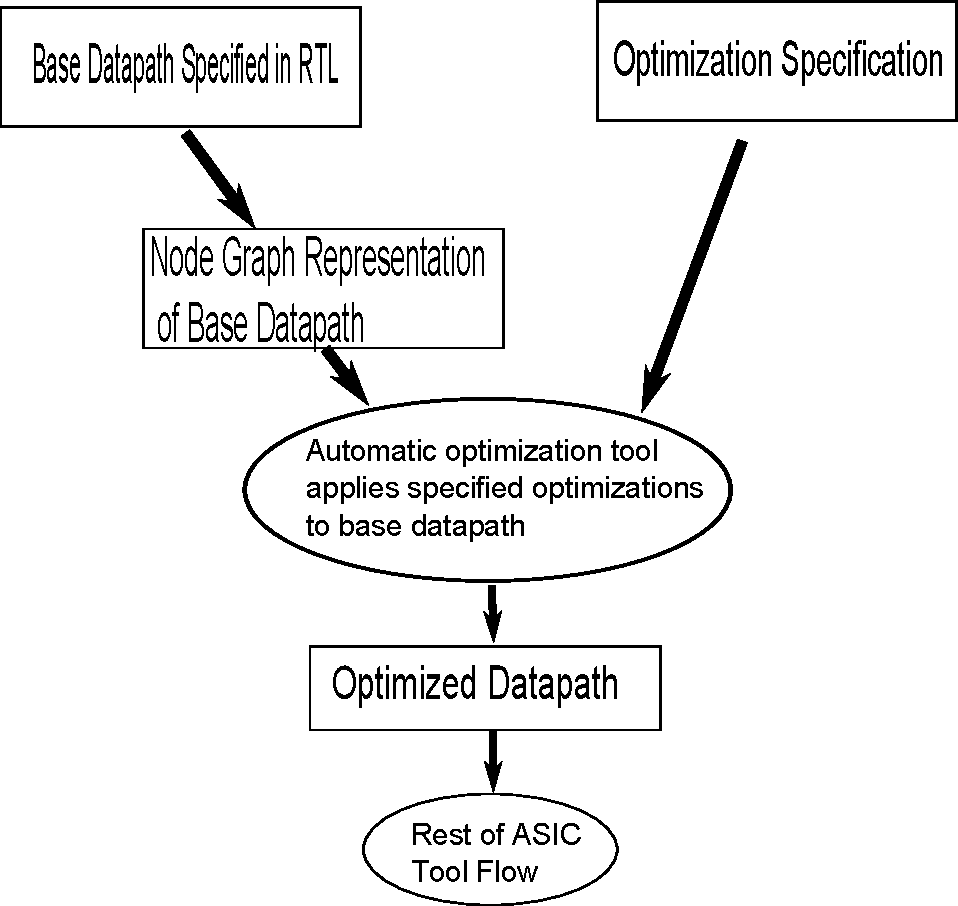
\includegraphics{figures/abstract-work-flow}}
    \caption{General Tool Flow}
	\label{fig:workflow}
\end{figure*}

\section{Proposed Solution}
HLS produces designs with unacceptable performance, power, and area characteristics because the synthesis tool has to solve the computationally difficult problem of formulating a datapath that executes the dataflow graph and fits within the given performance, power, and area constraints. HLS tools do synthesize well optimized designs for specific patterns that occur in the high-level specification, so hardware designers working with HLS find themselves tuning high-level code to make specific synthesis tools produce exactly the datapath they want. 

This is clearly a case of automation trying to do too much. The HLS tools have a hard time formulating optimized datapaths, so the designers have to essentially tell the HLS tools what datapath they should use in a roundabout way by tuning the high-level specification. Clearly, designers would be more productive if they can specify the datapath directly. 

It seems like this conclusion tells us that designers should just do logic design using RTL in the traditional manner. However, much of traditional RTL specification deals with issues outside of simple datapath design. Logic designers spend much of their time specifying additional logic required to make the datapath fit performance, power, and area constraints. Some common optimization techniques include time-multiplexing functional units, pipelining, multi-threading, out-of-order execution, etc. These commonly used datapath optimization techniques can be captured as algorithms and applied automatically.

This thesis proposes a system in which the designer creates a RTL specification of a functionally correct base datapath with no optimizations implemented and separately specifies a series of optimizations to be performed on the datapath. Then automatic tools that know how to generically apply common optimization techniques can apply the specified optimizations to the base functional datapath and produce an optimized gate level specification to be fed into the next step in the IC design flow which may be physical design, FPGA synthesis, or simulation. This work flow is shown in Figure \ref{fig:workflow}. This system of specification will hence be referred to as Automatic Functional Datapath Optimization (AFDO). AFDO allows the designer to specify a digital circuit with higher productivity than RTL specification without incurring the performance, power, and area penalties of HLS specification.

The automatic optimization tools discussed above work in the following manner. First, some initial processing transforms the RTL specification of the base datapath into a node graph data structure, where each node represents a digital circuit component (wire, combinational logic block, or state element) and each node contains input and consumer pointers to other nodes representing the topology of the circuit. Second, the tools implement the specified optimizations by modifying this node graph - creating new nodes, changing input/consumer pointers, copying existing nodes, etc. Third, the tool outputs the modified circuit in some specified representation.

Although AFDO can be implemented if the base datapath is specified in discrete event simulation based RTL languages such as Verilog or VHDL, it is better for the base datapath to be specified in a structural construction based RTL language such as Chisel. First, as mentioned in \ref{section:RTLCons}, discrete event simulator semantics are not particularly well suited for digital hardware specification and create a host of problems for the designer. Second, creating a node graph representation of the base datapath is much easier in structural construction based HDL languages such a Chisel as there is a one to one mapping between language construct and nodes in the node graph. In the case of Chisel, the automatic tools can directly operate on Chisel’s internal node graph data structure. In discrete event simulation based RTL languages, we have to first send the RTL specification through a gate level synthesis tool before we can construct the node graph data structure. This makes preserving names difficult and prevents the designer from using RTL level simulations of the automatically optimized designs. All of the automatic optimization tools discussed in the following sections apply transformations to base datapaths specified in Chisel or a reduced Chisel like RTL specifically designed to demonstrate AFDO that will be referred to as Scalpel.

AFDO increases logic designer productivity by addressing both limitations of RTL specification covered in \ref{section:RTLCons}. By using a structural construction based RTL language like Chisel to specify the base functional datapath, the problems caused by discrete event simulator semantics are eliminated. By allowing the designer to specify only the base functional datapath, which is generally much less complex than the optimized design, and applying optimizations automatically, source code verbosity and algorithm obfuscation is eliminated. Now the designer can specify designs much faster and with fewer errors as he only has to specify the simple base functional datapath and use automatic tools to systematically apply the desired optimizations. Additionally, AFDO allows designers to more easily do design space exploration as they can produce new design points by simply selecting different optimization options for the automatic tools to apply instead of rewriting obfuscated RTL for each new design point. For example, adding a pipeline stage to a processor design in RTL is generally non-trivial in RTL because the pipeline control logic is entwined within the datapath specification. If the designer specifies a base functional 1 stage version of the processor and uses an automatic tool to pipeline the processor, adding a pipeline stage would be trivial on the part of the designer as he would simply have to tell the automatic pipeline tool to generate one more stage.

At the same time, AFDO retains performance, power, and area benefits of RTL specification by preserving a high level of correlation between language constructs and the generated hardware. The generated datapath is simply the base functional datapath modified with the designer specified optimizations. Unlike HLS, the designer knows the number and types of functional units used in the datapath as well as the state elements that are present in the datapath along with how those state elements are updated.
